\section{Experimental Setup}\label{sec:exp-dataset}

We use Bitcoin Core software\footnote{https://bitcoin.org/en/bitcoin-core/} to run full node \bc clients on 5 virtual machines on a campus network. Each virtual machine is connected to the Internet with high bandwidth. Before starting the experiments, we leave our \bc clients for a few days to make sure they have downloaded an up-to-date blockchain ledger. The \bc client is passively receiving blocks and participating in the Bitcoin network, but it is not doing any transactions.
We capture \bc traffic under three different scenarios on a Linux $16.0.4$ virtual machine: 
%Following explains the traffic that we capture:
%\begin{compactitem}
\subsection{Datasets}
\paragraphb{Collecting \bc traffic:} We use \bc version 0.12.0 to capture \bc traffic in the full block relaying mode and Bitcoin version 0.14.0 to capture traffic in the compact block relaying mode. We capture \bc traffic for each version for a period of a month.
%Specifically, we captured the Bitcoin traffic in the full block relaying mode from August 28th to October 9th, 2016,  and \bc traffic in the compact block mode from March 14th to April 18th, 2017.

\paragraphb{\bc tunneled through Tor} We captured \bc traffic behind Tor~\cite{tor} for both compact and full block modes.
We also captured \bc traffic in the compact block mode behind %OpenVPN\footnote{https://openvpn.net/}, 
Tor and popular Tor pluggable transports of obfs4~\cite{obfs4}, FTE~\cite{fte}, and Meek-amazon~\cite{meek}.
%Furthermore, we capture \bc traffic tunneled through . 

\paragraphb{\bc with background traffic:} We captured \bc traffic in presence of HTTP background traffic by browsing the top 500 Alexa websites using the Selenium\footnote{\url{http://www.seleniumhq.org}} tool while running \bc software. We also collected \bc 
traffic with HTTP background for the same set of websites behind Tor and its three pluggable transports using Selenium.

\iffalse  \textbf{\bc traffic } in full and compact mode(30 days each). Also, \bc compact mode traffic over VPN, Tor and three pluggable transports(up to 20 days)\fi

\paragraphb{CAIDA background traffic:}
We use CAIDA's 2018 anonymized traces\footnote{\url{https://www.caida.org/data/monitors/passive-equinix-nyc.xml}} as a dataset for additional background traffic. 
%We extracted the flows in this database based on the protocol type, IP addresses and port numbers of the end-hosts. 
%For each IP address, we consider all traffic to and from that IP as the typical traffic of that user. Table~\ref{tab:traffic_class} shows the class breakdown of CAIDA dataset used in our experiments.

\paragraphb{HTTP traffic:}% (normal traffic, behind VPN and Tor)
We collect top $500$ Alexa websites using Selenium tool. Also, we capture these websites over Tor, and three pluggable transports. Moreover, we use 
the dataset by~\cite{deepcore} which has collected the top $50,000$ Alexa websites over Tor. 


%\end{compactitem}

\iffalse
\begin{figure}[!t]

\begin{subfigure}{.48\linewidth}
\centering
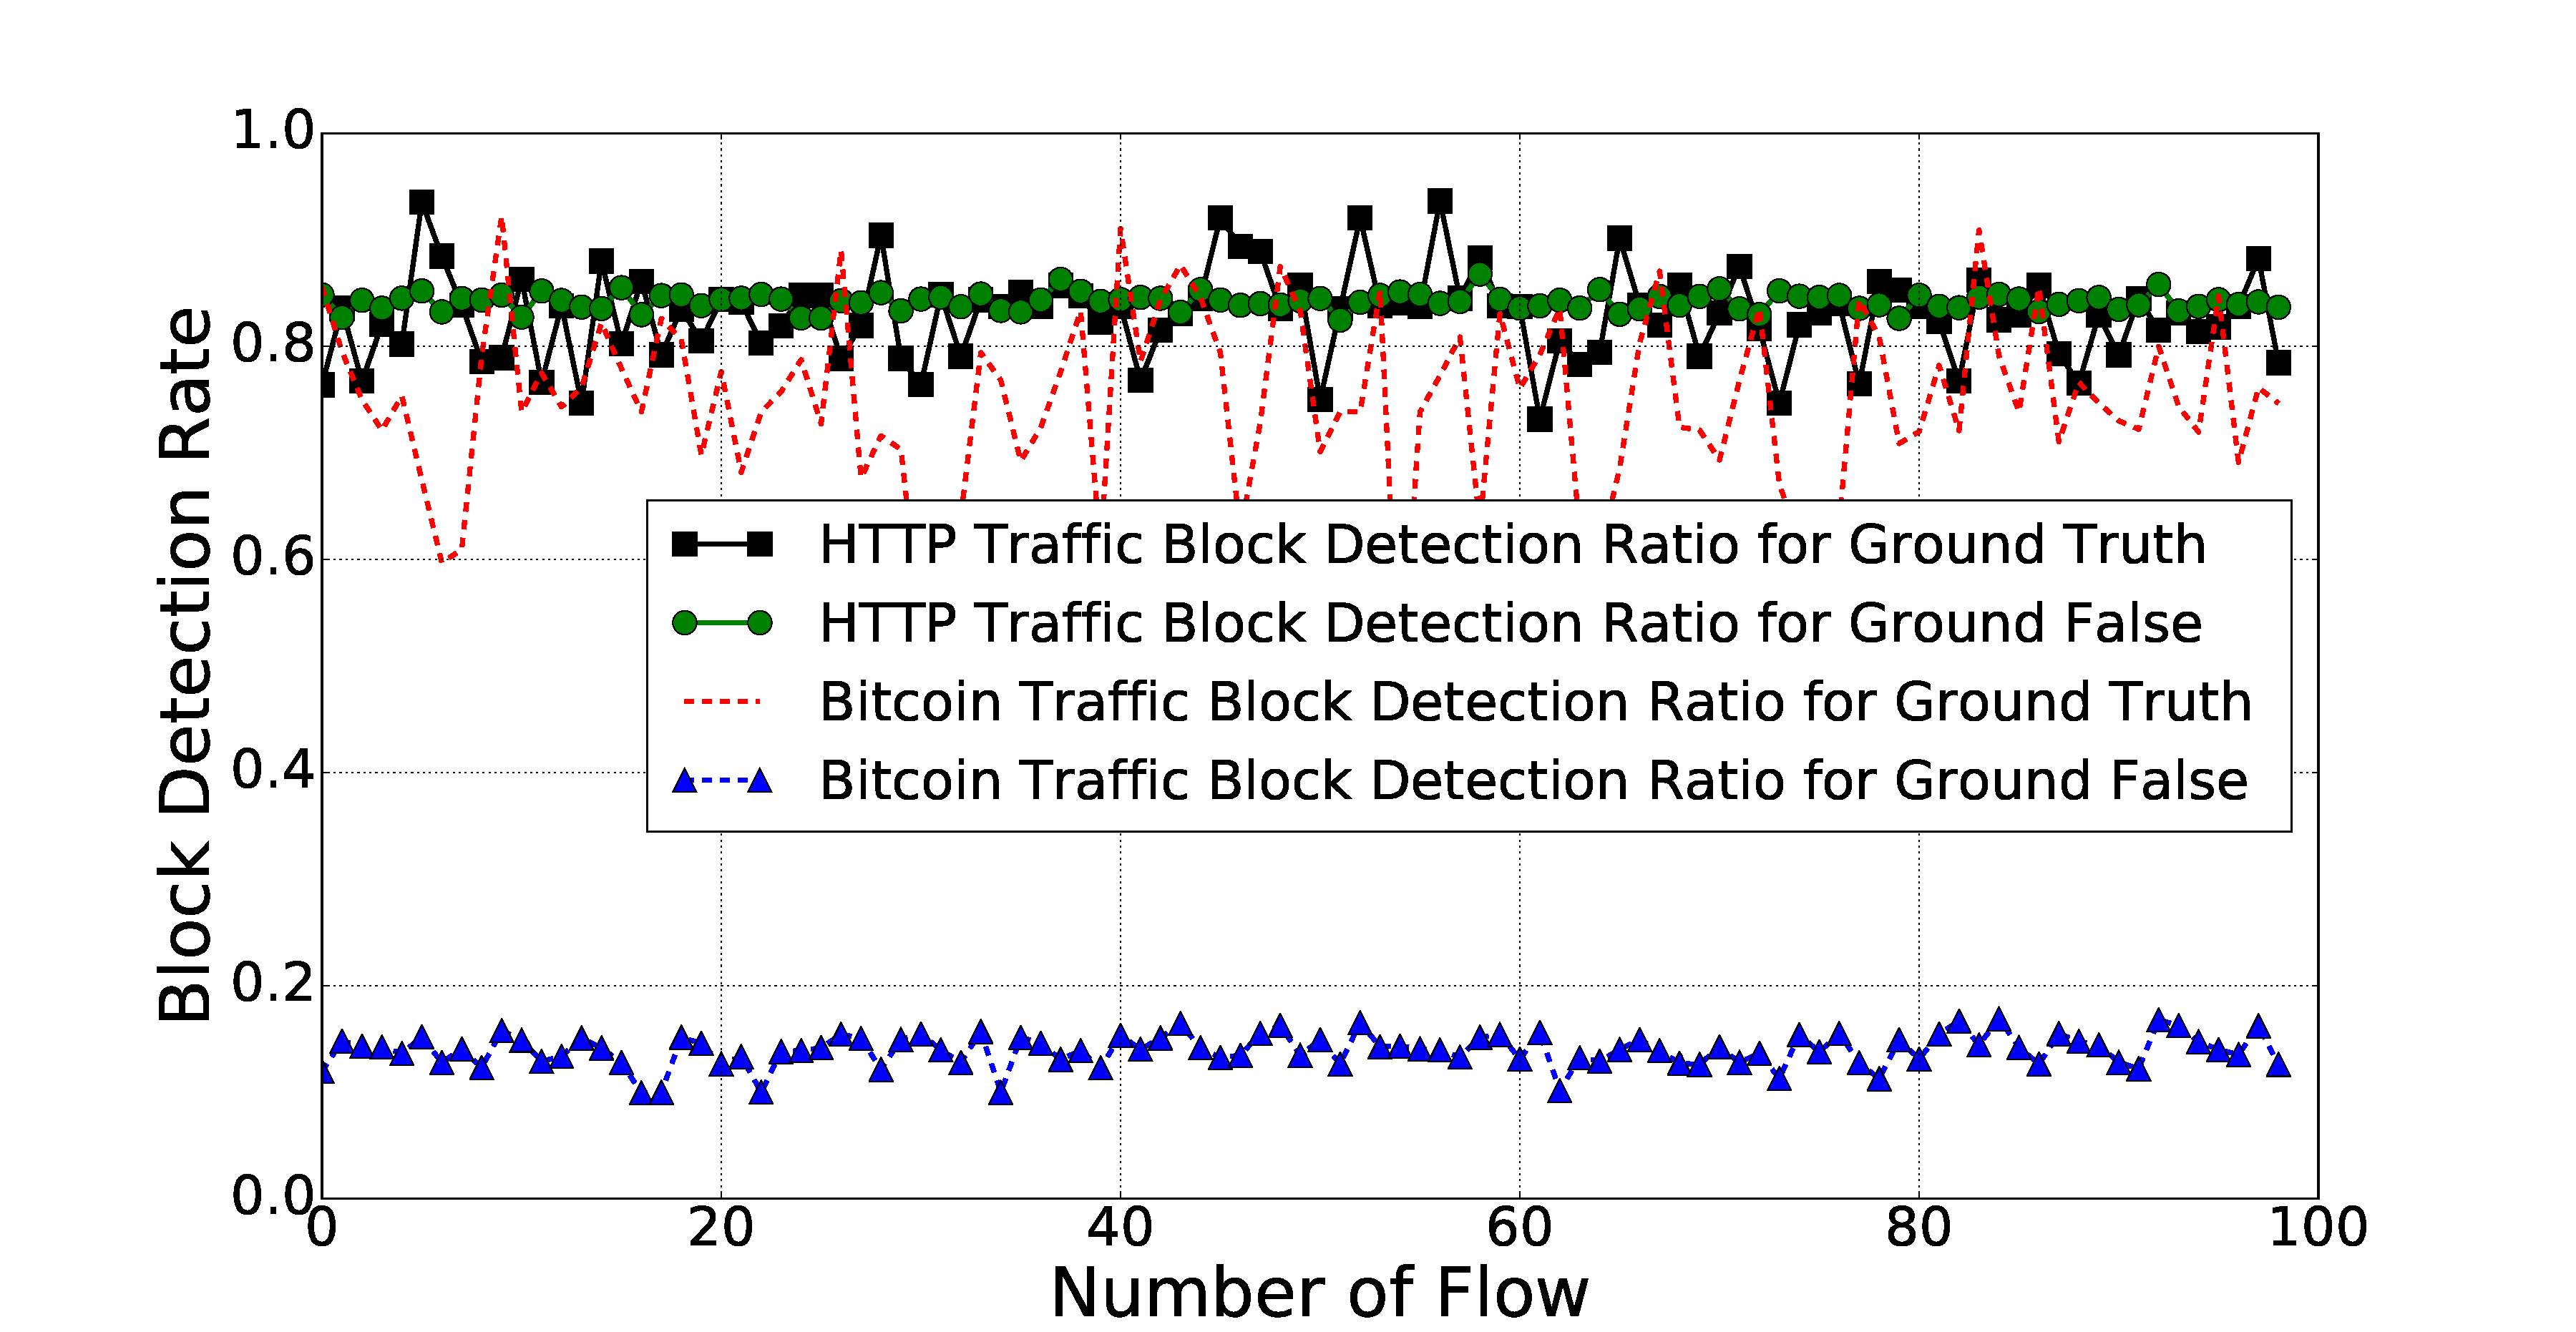
\includegraphics[width=\linewidth]{image/nov7/window/bc_http_window.pdf}
\caption{Detection Rate for Ground True and False}
\label{fig:gft_wind}
\end{subfigure}
\centering

\begin{subfigure}{\linewidth}
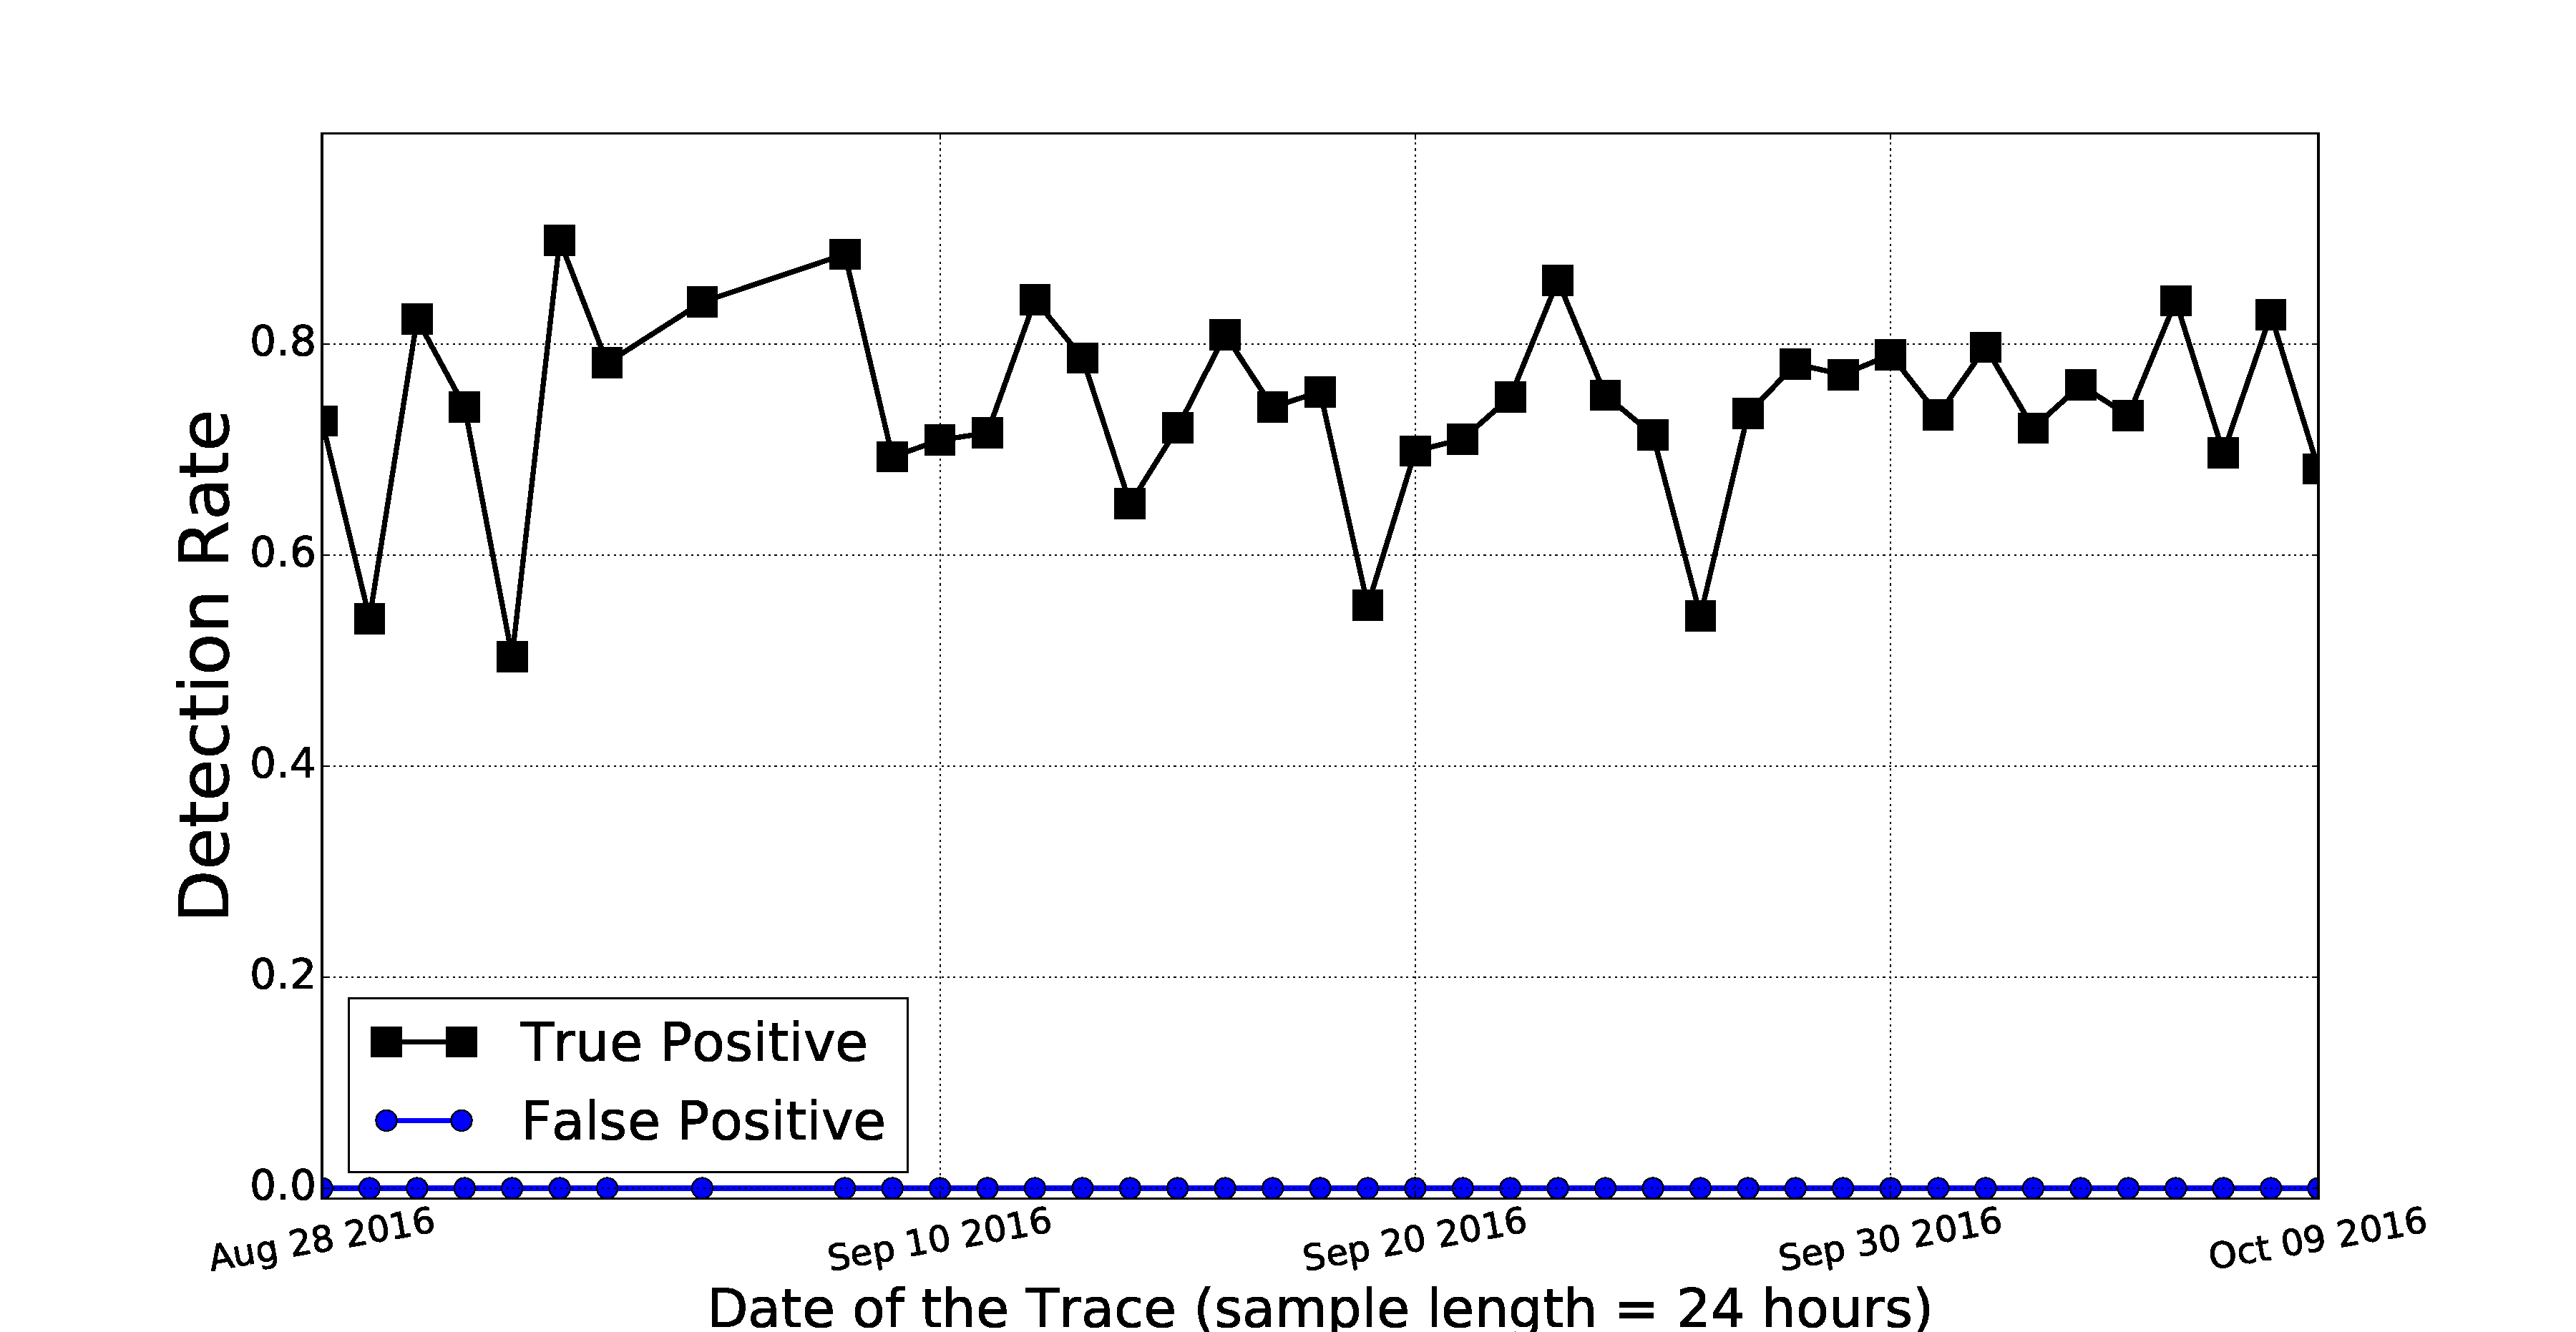
\includegraphics[width=\linewidth]{image/nov7/window/window.pdf}
%\caption{Result on full block mode}
\label{fig:res_wind}
\end{subfigure}
\caption{Window-based classifier}
\label{fig:window}
\end{figure}
\fi

\begin{comment}
 \begin{table}[h!]
  \begin{center}
    \caption{Traffic Class Breakdown For CAIDA Dataset}
    \label{tab:traffic_class}
    \begin{tabular}{c|c|c|c}
     \textbf{Traffic Class}& \textbf{Port Numbers} &\textbf{$\sharp$ of 			  Connections}&\textbf{$\%$of Total}\\
      \hline
		http, https& $80, 8080, 443$&745262&$0.318$\\
		dns& $53$&1073758&$0.457$\\
		smtp& $25$&2646&$0.001$\\
		telnet&$23$&6958&$0.003$\\
		ssh/scp&$22$&4928&$0.002$\\
		other&$-$&511700&$0.219$\\
		\hline
		all &&2345252&1.0\\
		\hline
    \end{tabular}
  \end{center}
\end{table}
\end{comment}

\begin{table}
\center \caption{Traffic class breakdown for CAIDA dataset}\label{tab:traffic_class}
\begin{tabular}{|c|c|c|c|}
\hline
 Traffic class& Port numbers &Number of connections&$\%$of total\\
      \hline
		http, https& $80, 8080, 443$&745262&$0.318$\\
		dns& $53$&1073758&$0.457$\\
		smtp& $25$&2646&$0.001$\\
		telnet&$23$&6958&$0.003$\\
		ssh/scp&$22$&4928&$0.002$\\
		other&$-$&511700&$0.219$\\
		all &$-$&2345252&1.0\\
\hline
\end{tabular}
\end{table}

\subsection{Metrics}

We use following metrics to measure the performance of our classifiers:
\begin{compactitem}
\item \textbf{True positive:} True positive shows the proportion of the data which contain \bc, and our model correctly identified as \bc traffic.
\item \textbf{False positive:} False positive shows the proportion of the data which did  not contain \bc traffic, and our model incorrectly classified as \bc.
\item \textbf{Accuracy:} Accuracy shows the proportion of the data which was correctly classified.
\end{compactitem}
\begin{figure*}

\begin{subfigure}{0.48\linewidth}
\centering
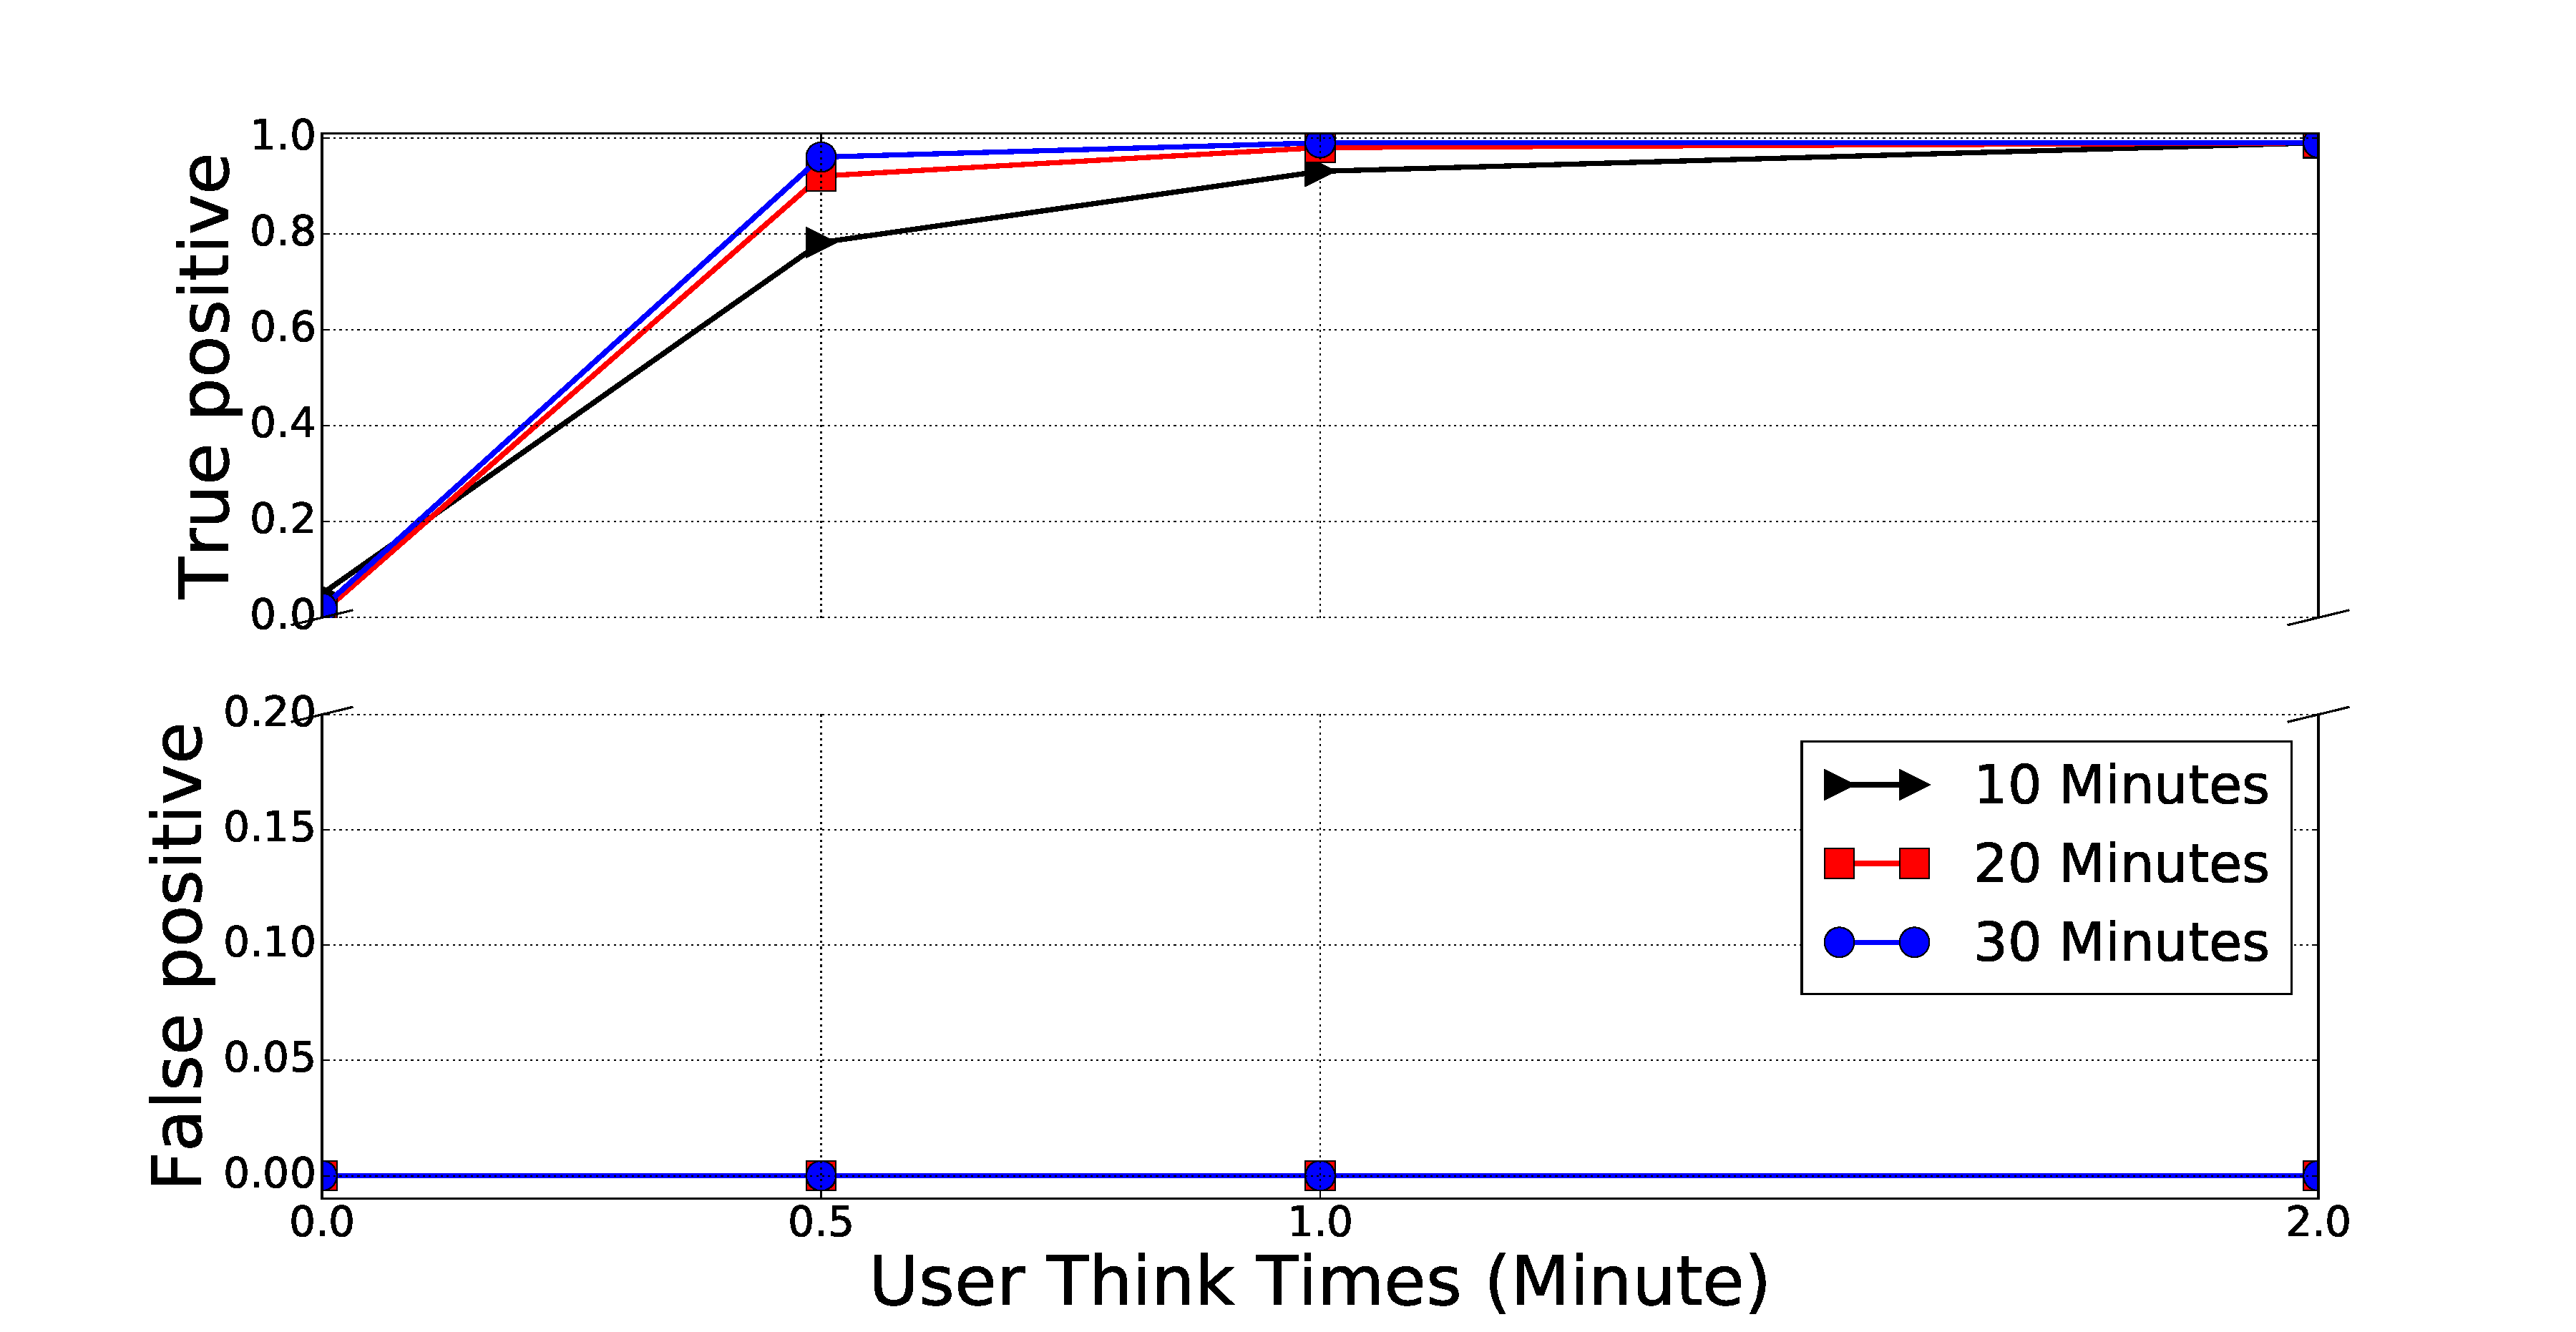
\includegraphics[width=\linewidth]{image/jan25/cmp_sizeHist.pdf}
\caption{Compact Mode}
\label{fig:vanilla_sizeTor}
\end{subfigure}
\begin{subfigure}{0.48\linewidth}
\centering
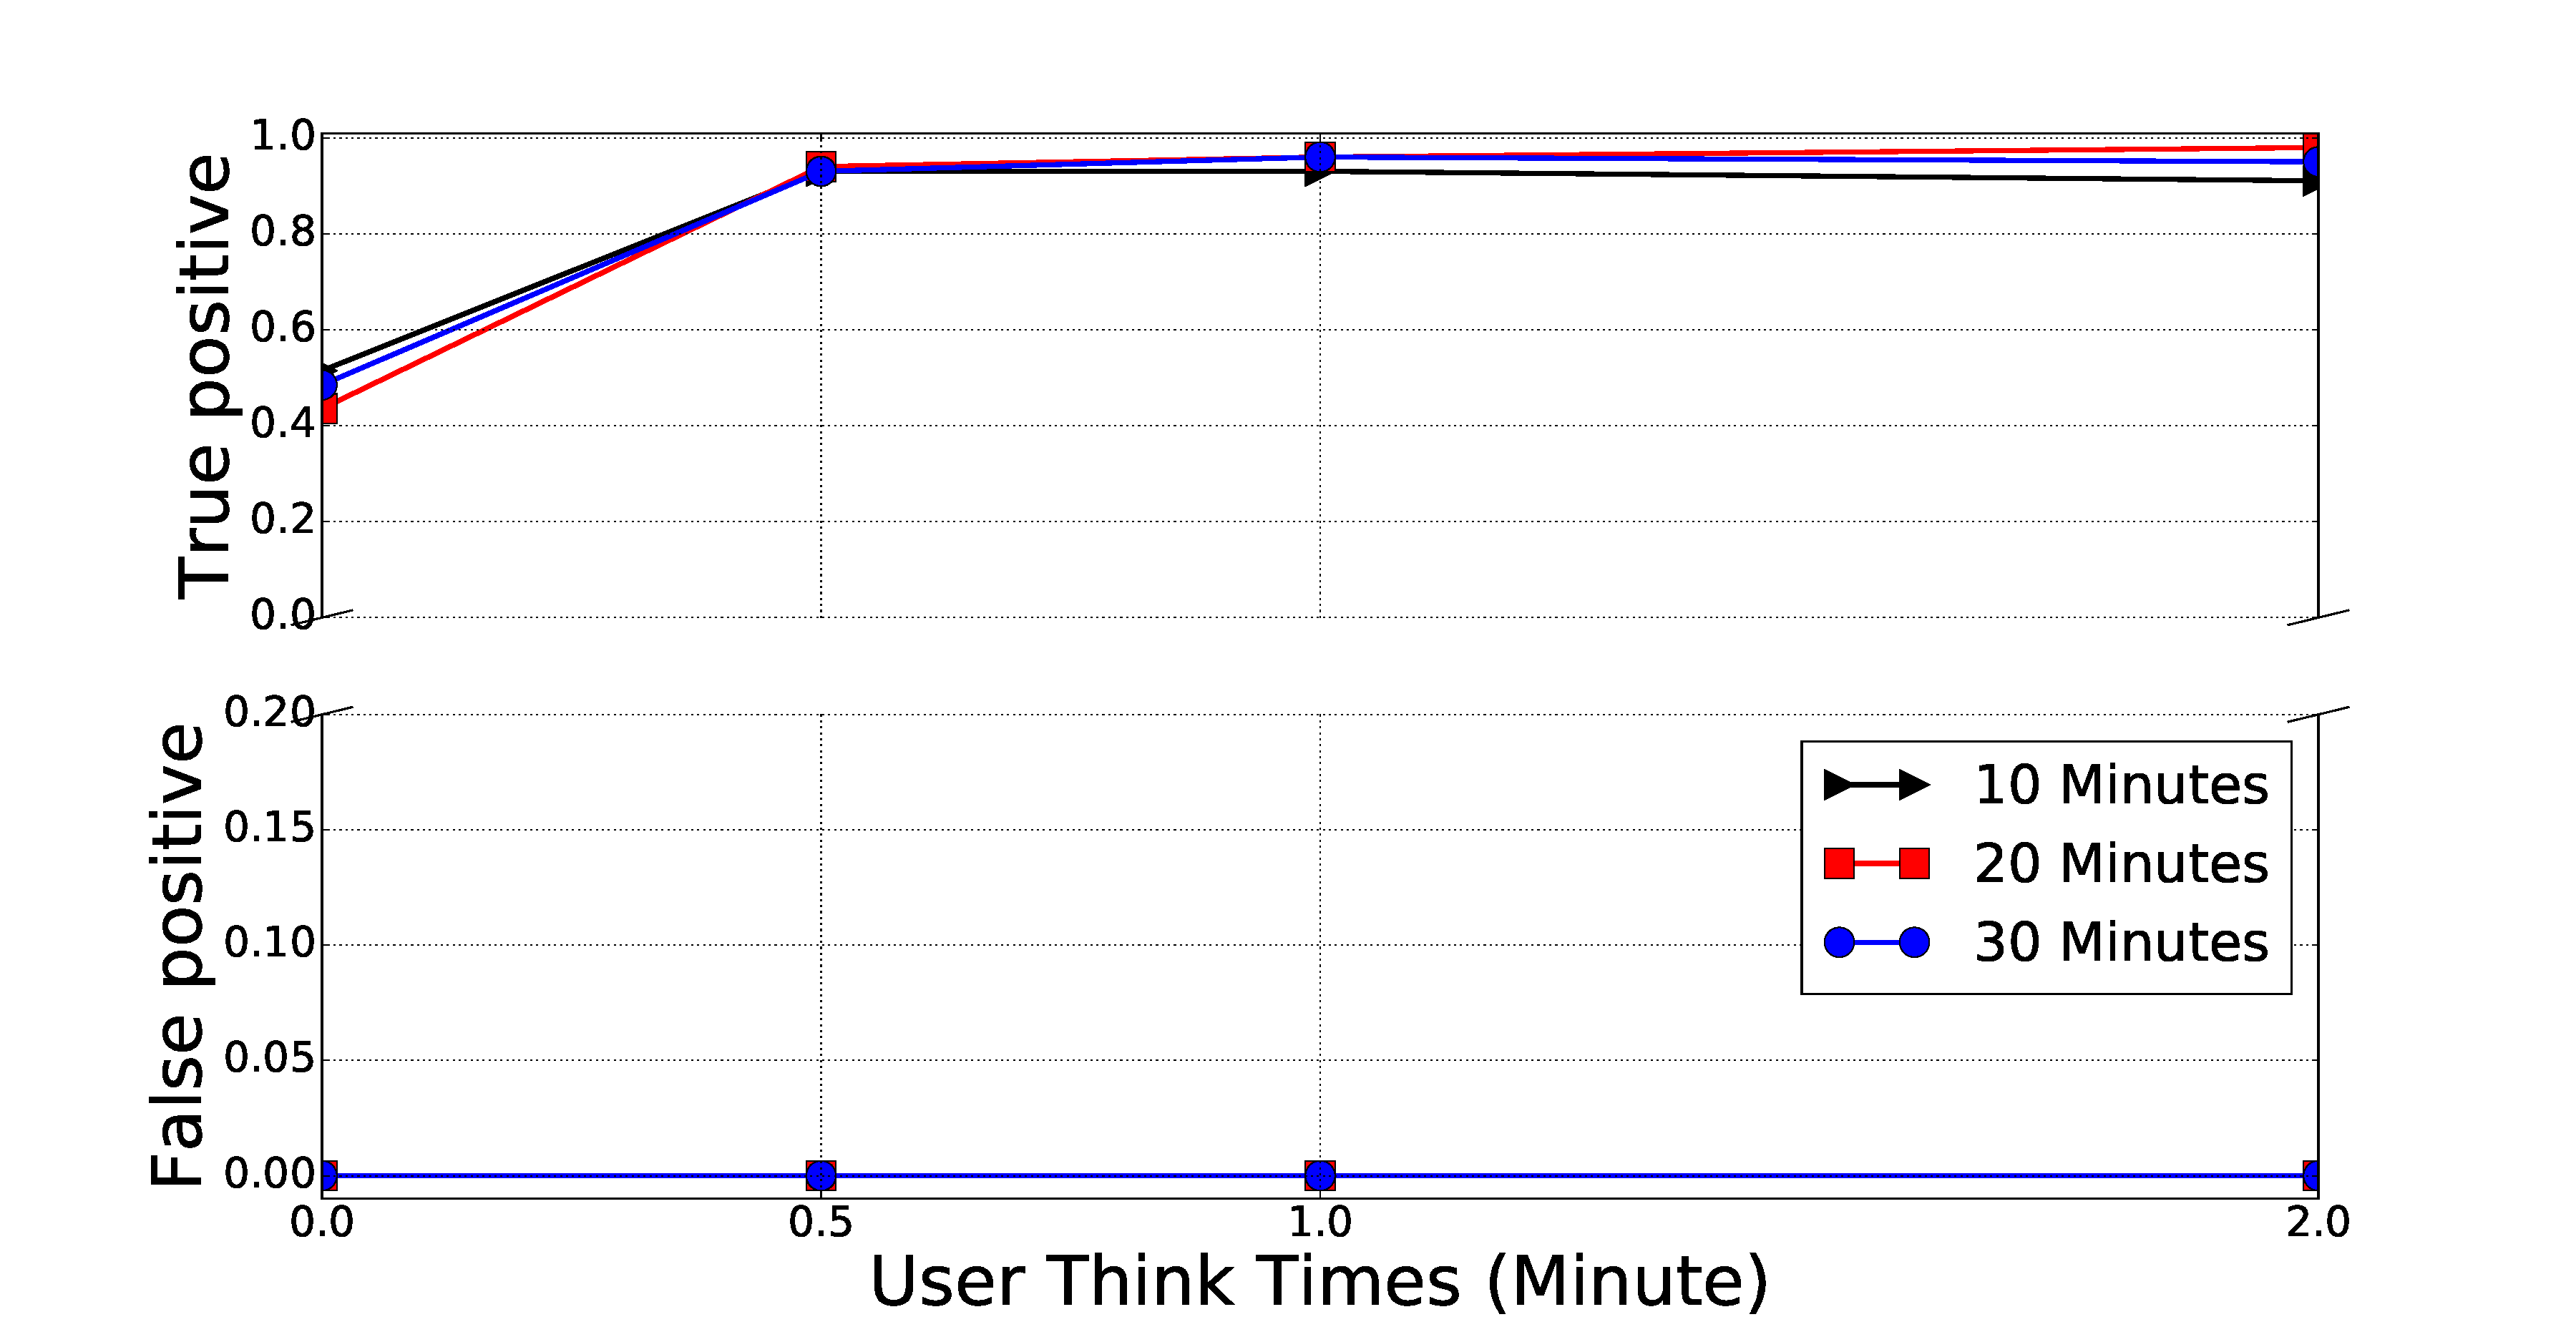
\includegraphics[width=\linewidth]{image/jan25/full_sizeHist.pdf}
\caption{Full Mode}
\label{fig:vanilla_d2u}
\end{subfigure}
\caption{Result of \code{sizeHist} classifier on noisy Bitcoin traffic}
\label{fig:sizeHist_non}
\end{figure*} 
\subsection{Modeling Normal Users}\label{simpleuser}

In this section, we describe four different types of users' profile that we use to evaluate the performance of our \bc classifiers against.% Users may have some background traffic while using Bitcoin or they can generate noisy traffic to evade detection. Therefore, we attempt to model typical behavior of users in various scenarios, and apply each classifier on one or more number of these profiles to evaluate their performance.

\begin{itemize}
    \item Simple User: A simple user is a Bitcoin client with no background noise and traffic. This type of user does not generate any network traffic except the Bitcoin client application traffic. Therefore, all traffic of the simple user is Bitcoin traffic. 
    \item Simple Noisy User: A simple noise user is a \bc client who browses only \textbf{one} webpage.% In some cases, she may run the Bitcoin client as well. 
    To control the background traffic, we introduce a parameter named think time, T, representing the amount of time that the user spends on a particular website. %Note that, increasing T would decrease the background noise since there is not much traffic after a website is loaded. Thus, if T is large and the Bitcoin application is running, after the webpage is completely loaded, the simple noisy user's traffic would look like the simple user's traffic.
    \item Complex Web (Complicated/Sophisticated) User: A complex user is a \bc client who browses \textbf{multiple} websites simultaneously.
    
     %Similar to the simple noisy user, she may run the Bitcoin application besides web surfing.% The user has the ability to use Tor to hide all of her traffic consisting of the Bitcoin and web traffic but she may decide not to use Tor. Thus, she can choose to pass all or none of her traffic over Tor and not some of it. 

\begin{comment}
    The complex web user is the sophisticated version of the simple noisy user. 

To create a sample data of this user profile, we choose a \bc traffic with length of sample size and accumulate the noise traffic using following algorithm: 
\begin{enumerate}
 \item Choose a random number ($k$) in the range $[0$, \textit{sample size}$]$, which represents
 the length of noise flow. 
 \item  Choose another random number ($p$) in the range $[0$,  \textit{sample size}$ - k]$, which shows where we
 need to add the noise: p's second of the \bc traffic.
 \item Repeat 1.
\end{enumerate}
We repeat this process for $I$ number of times, which represents the number of open tabs. The reason that we do not add noise from start to the end of the flow is that we want to make the background noise nonuniform, thus prevent the classifier from learning the noise and denoising the traffic.\end{comment}
    \item Complex CAIDA User: A complex CAIDA user is a \bc client who is running 1-5 number of CAIDA applications, which is introduced in table 2 simultaneously in the background. %We use the same algorithm as above to create this user profile.
\end{itemize}    
%We define four different user profiles from simple behavior to more realistic and complicated ones. 


\begin{comment}

In this section, we describe the type of users that we use to evaluate the performance of our \bc classifiers.
\subsubsection{User profiles for SizeHist and D2U classifiers}\label{binary_user_noise}
We consider two user profiles to evaluate the performance of our \bc classifiers in simple scenarios. First scenario is a \bc user who has no background noise. 
\begin{compactitem}
\item Simple User: A \bc client with no background noise.
\item Noisy User: A \bc user who is browsing Internet on the background. To control the background traffic, we introduce a parameter named \textit{think time}, T, which represents a time that user spends on a particular website. Note that, increasing T would decrease the background noise Since there is not much traffic after a website is loaded.
\end{compactitem}


\subsubsection{User model for NN-based and SizeTor classifiers}\label{setup:nn}
Here, we expand the user profiles in the previous section to have a more realistic scenario to evaluate our NN-based and SizeTor classifiers.%We generate a large corpus of data consisting of a user with $2-5$ number of open tabs. Also, a user who is running one or more number of applications -introduced in table~\ref{tab:traffic_class}- at the same type.

\begin{compactitem}

\item Complex User-1: A user who is browsing the Internet and browses multiple websites simultaneously. To create this user profile, we accumulate traffic from different websites. For example, for a background noise of two tabs, we add the traffic of two different websites.

\iffalse and has $2-5$ number of open tabs (she can be a \bc client as well). Since this model represents a user with
larger background noise, we consider $T$ to be $0$ seconds. Note that each open tab represents a single layer of background noise. We create each layer of background noise using the following algorithm:
\fi
 

 \item Complex User-2: A user who is running $1-5$ number of applications simultaneously, which is introduced in table ~\ref{tab:traffic_class} (she can also be a \bc client). 
\end{compactitem}
Therefore, we have $4$ type of users: complex User-1 with and without \bc, and complex User-2 with and without \bc. We add these user types to the previous ones to create a big corpus of data for our NN-based and SizeTor classifiers.
\end{comment}
